In diesem Experiment wird gezeigt, dass obwohl ein Agent sein Ziel schon erreicht hat, immer noch aktiv an der passiven Kooperation teilnimmt.

\textbf{Aufbau des Experiments}
\begin{figure}[H]
    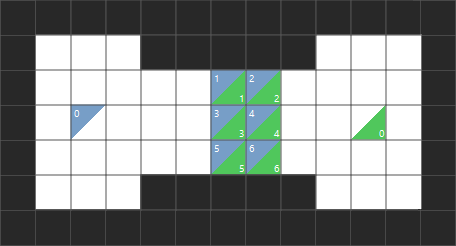
\includegraphics[height=56mm]{images/crowd_drive-through.png}
    \centering
    \caption{Aufbau für das Durchfahren eines Agenten durch ein Menge stehender Agenten}
    \label{fig:menge}
\end{figure}
Die Abbildung \ref{fig:menge} zeigt die Karte für dieses Experiment. Diese hat Dimensionen von elf mal fünf Felder. In der Mitte ist eine fünf Felder lange und drei Felder breite Engstelle. In dieser Engstelle stehen in zwei Reihen hintereinander sechs Agenten. Die Startpositionen dieser Agenten sind gleichzeitig ihre Zielpositionen. Ein weiterer Agent hat seine Startposition auf der linken Seite der Engstelle und seine Zielposition auf der Rechten. Er muss also durch die stehende Menge, um sein Ziel zu erreichen.

\textbf{Erwartete Beobachtungen}\newline
Die Agenten "'3"' und "'4"' werden von Agent "'0"' verdrängt, fahren also von ihren Zielpositionen weg, um Platz für Agent "'0"' zu machen. Es ist auch möglich, dass dabei andere Agenten von ihren Zielpositionen verdrängt werden. Nachdem Agent "'0"' die Menge durchquert hat, fahren alle Agenten wieder zurück zu ihren Zielpositionen.